\section{Исследование поведения концов блужданий модели RW}

Следующие разделы посвящены исследованию поведения частного случая локального координационного числа на конце блуждания, или ''атмосфере'' блуждания. 
В качестве основной наблюдаемой берётся $\pkn$ -- вероятность существования блуждания с количеством шагов $N$ с атмосферой $k$.
Атмосферу блуждания можно легко посчитать как разность координационного числа решётки (для квадратной - 4) и локального координационного числа (число соседей вокруг узла) на конце блуждания.
В рамках симуляций Монте-Карло данная наблюдаемая считается среди сгенерированной выборки:

\begin{large}

\begin{equation}
\begin{array}{l}
a_t = 4 - c_{\textup{end}}(t), \\
\pkn = \frac{\sum_{t=0}^{\textup{M}} [a_t = k]}{\textup{steps}},
\label{eq:pkn}
\end{array}
\end{equation}

\end{large}
где $c_{\textup{end}}(t)$ -- число соседей на конце t-го сгенерированного блуждания, $\textup{M}$ -- объём сгенерированной выборки, а $a_t$ -- атмосфера t-го сгенерированного блуждания. Пример подсчёта атмосферы блуждания изображен на рисунке \ref{fig:path_atm}.

Ранее исследование данного свойства проводилось в работе \cite{owczarek2008scaling}, на невзаимодействующих случайных блужданиях без самопересечений. 
Так же подобная задача рассматривалась в книге \cite{Spitser1969}, на странице 206 под номером 9, для \textit{возвратного простого случайного блуждания}. Задача формулируется следующим образом:

\begin{itemize}
    \item Случайное блуждание на квадратной решётке начинается из некоторой точки $x_0 = \chi$, не лежащей в начале координат.
    \item Процесс случайного блуждания длится не фиксированное количество шагов, а до фиксированной \textit{точки остановки} - до достижения блужданием начала коордиинат $x_{\textup{end}} = 0$
    \item До достижения точки остановки блуждание может посетить одну или несколько соседних с ним точек - (0,1), (1,0), (0,-1), (-1,0). Пусть число уникальных посещенных блужданием соседних точек  $N \in \{1, 2, 3, 4\}$
    \item Задачей является вычислить вероятности блуждания посетить каждое возможное количество уникальных соседних точек для бесконечно удаленной от начала координат начальной точки блуждания $\chi$:
    
    \[ p_{n} = \lim_{|\chi|\to \infty} P_{\chi}[N = n] =\ ?,\ \ \ n = 1, 2, 3, 4\]
\end{itemize}

Так же в качестве подсказки было указано, что отношение $p_1:p_2:p_3:p_4$ почти равно $4:3:2:1$.
Пример возвратного блуждания с точкой остановки в начале координат изображен на рисунке \ref{fig:path_spitser}. 

\begin{figure}[h]
    
\begin{subfigure}{0.5\textwidth}
    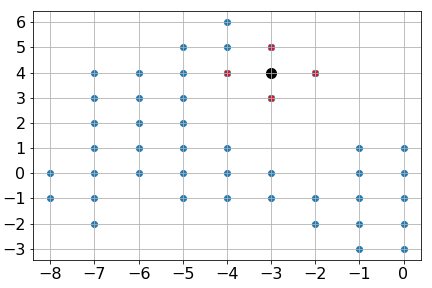
\includegraphics[width=\textwidth]{Rand_Path_Atm.png}
    \caption{}
    \label{fig:path_atm}
\end{subfigure}
\hfill
\begin{subfigure}{0.5\textwidth}
    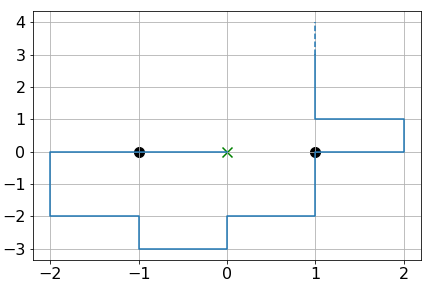
\includegraphics[width=\textwidth]{Spitser.png}
    \caption{}
    \label{fig:path_spitser}
\end{subfigure}
\caption{а) Подсчёт атмосферы блуждания модели RW (продолжение рисунков \ref{fig:path_alg}). Для данного блуждания все соседние узлы его конца уже посещены ранее, атмосфера блуждания $a=0$. b) Пример исследуемого блуждания в задаче \cite{Spitser1969}: из бесконечно удаленной точки (движение отмеченно пунктиром) блуждание посетило две соседние началу координат точки (отмечены чёрным), прежде чем остановилась в нём (точка остановки отмечена зелёным крестиком).}
\end{figure}



В рамках летней производственной практики (см. Отчёт о практике) задача из работы Спитцера была теоретически и экспериментально решена. 
Результаты расчётов можно увидеть в таблице \ref{tab:Spitser_res}:

\begin{table}[h]
	\centering
	\begin{tabular}{|c|c|c|c|c|}
	\hline
	$p_1$ &  $p_2$ & $p_3$ &  $p_4$ \\ \hline
 	0.393566 & 0.314680 & 0.190025 & 0.101729 \\ \hline
	\end{tabular}
	\caption{Аналитическое решение задачи из работы  \cite{Spitser1969}}
	\label{tab:Spitser_res}
\end{table}

В разделе \ref{sec:ni_scale} были найдены пределы долей узлов с фиксированным числом соседей $n_i$ \eqref{eq:n_i}.
Задачей следующих разделов, аналогично исследованию долей $n_i$, будет определение характера шкалирования $\pkn$ \eqref{eq:pkn}, оценка коэффициентов шкалирующих функций, а так же сравнение асимптотических пределов вероятностей $\pkn$ при стремлении числа шагов блуждания к бесконечности ($N \to \infty$):

\begin{enumerate}
\item с ответами на ранее описанную задачу \cite{Spitser1969}
\item с найденными в разделе \ref{sec:ni_scale} пределами долей $n_i$ \eqref{eq:n_i} (таблицы \ref{tab:n_i_log_log} и \ref{tab:n_i_u_log_log})
\end{enumerate}

\newpage

\subsection{Зависимость атмосфер от количества шагов блуждания и уникальных узлов}

Была рассчитана вероятность блуждания модели RW фиксированной длины $N$ иметь атмосферу $k$. 
Под длиной блуждания $N$ здесь имеется в виду количество случайных шагов, проделанных блужданием, без учёта, сколько уникальных узлов оно занимает.
Результаты можно увидеть в таблице \ref{tab:randw_p_atm} и на графиках \ref{fig:randw_p_atm}, как функции от $N$, и \ref{fig:randw_p_atm_u}, как функции от $\Nun$.

\begin{figure}[h]
    
\begin{subfigure}{0.49\textwidth}
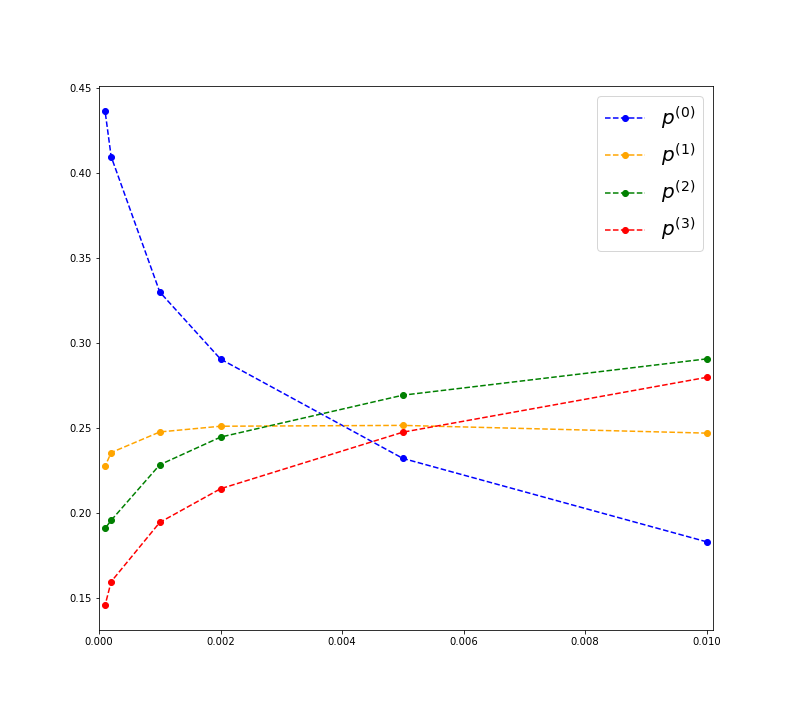
\includegraphics[width=\textwidth]{randwalk_p_atmos.png}
\caption{}
\label{fig:randw_p_atm}
\end{subfigure}
\hfill
\begin{subfigure}{0.49\textwidth}
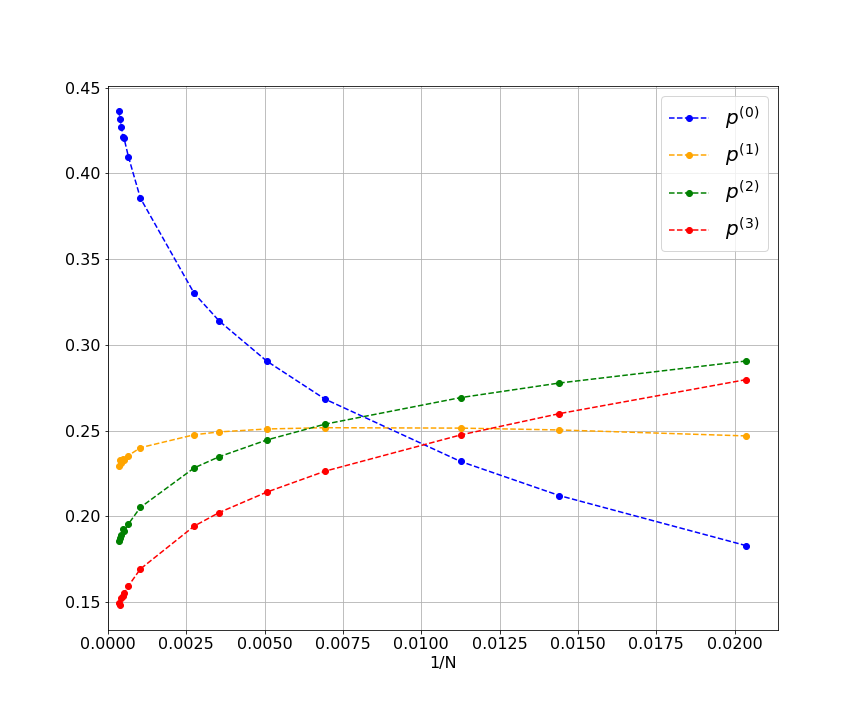
\includegraphics[width=\textwidth]{randwalk_p_atmos_unique.png}
\caption{}
\label{fig:randw_p_atm_u}
\end{subfigure}
\caption{Вероятность конформации модели RW  иметь атмосферу k=0,1,2,3  (столбцы $p^{(0)}$-$p^{(3)}$ из таблицы \ref{tab:randw_p_atm}): от a) от обратного количества шагов $1/N$ (столбец $N$); b) от обратного количества уникальных узлов $\Nun = N\nun$.}
\end{figure} 

\begin{table}[h] 
\centering
\begin{tabular}{|c|c|c|c|c|c|c|}
\hline
N & M & $ \nun $ & $p^{(0)}$ & $p^{(1)}$ & $p^{(2)}$ & $p^{(3)}$ \\ \hline
100 & 96430000 & 0.490868(8) & 0.182831 & 0.246855 & 0.290593 & 0.279720 \\ \hline
150 & 69360000 & 0.462622(9) & 0.212044 & 0.250342 &0.277737 &0.259877 \\ \hline
200 & 36140000 & 0.44436(1) & 0.231971 & 0.251413 & 0.269204 & 0.247413 \\ \hline
350 & 17070000 & 0.41251(2) & 0.268341 & 0.251656 &0.253724 & 0.226279 \\ \hline
500 & 7720000 & 0.39439(2) & 0.290471 & 0.250914 & 0.244515 & 0.214100 \\ \hline
750 & 4810000 & 0.37559(2) & 0.313906 & 0.249196 & 0.234730 & 0.202167 \\ \hline 
1000 & 2480000 & 0.36325(3) & 0.329962 & 0.247547 & 0.228218 & 0.194273 \\ \hline
3000 & 420000 & 0.32265(6) & 0.385626 & 0.239993& 0.205155 & 0.169226 \\ \hline
5000 & 140000 & 0.30679(9) & 0.409736 & 0.235407 & 0.195493 & 0.159364  \\ \hline
6500 & 100000 & 0.2992(1) & 0.420400 & 0.232740 & 0.191620 & 0.155240 \\ \hline
7000 & 305000 & 0.29610(6) & 0.421036 & 0.233311 & 0.192348 & 0.153305  \\ \hline
8000 & 240000 & 0.29338(6) & 0.427387 & 0.230854 & 0.189233 & 0.152525 \\ \hline
9000 & 195000 & 0.29022(7) & 0.431959 & 0.232795 & 0.187205 & 0.148041 \\ \hline
10000 & 160000 & 0.28751(8) & 0.436369 & 0.229075 & 0.185300 & 0.149256 \\ \hline
\end{tabular}
\caption{Результаты экспериментов, описанных на графиках \ref{fig:randw_p_atm} и \ref{fig:randw_p_atm_u}: столбцы $p^{(0)}$-$p^{(3)}$ показывают среднюю вероятность блуждания модели RW с количеством шагов $N$ иметь атмосферу 0-3 соответственно, объём сгенерированной выборки блужданий для каждой длины записан в столбце $M$.}
\label{tab:randw_p_atm}
\end{table}

Первичное рассмотрение графиков зависимости вероятностей от обратной длины $1/N$ в линейной, лог-линейной и лог-логарифмической масштабностях показало, что график лучше всего выпрямляется в третьем случае. 
Аналогичный результат показали графики остальных вероятностей, как функций от $N$ так и от $\Nun$.
Поэтому для всех четырех вероятностей аппроксимирующая функция при $N \to \infty$ ищется так же, как и для долей узлов, в двух видах - сначала как функция от количества шагов блуждания $N$, по формуле \eqref{eq:pi_N}.

\begin{equation}
p^{(i)}(N) = k_i * (1/N)^{a_i} + b_i, \ \ \ i \in \{ 0,1,2,3\} \\
\label{eq:pi_N}
\end{equation}

где $k_i$ - линейный наклонный коэффициент, $a_i$ - степенной коэффициент, а $b_i$ - свободный коэффициент. 
Оно же является пределом вероятности $p^{(i)}$ при $N \to \infty$.
Для поиска коэффициентов использовался метод наименьших квадратов.
Результаты апроксимации графиков вблизи $1/N = 0$, диапазон выбранных длин цепочек для подбора функции,
а так же стартовое положение описаны в таблицах \ref{tab:p_i_log_log} и \ref{tab:p_i_u_log_log}. 

\begin{table}[h] 
\centering
\begin{tabular}{|c|c|c|c|c|c|}
\hline
 & $k_i$ & $a_i$ & $b_i$ & N & start  \\ \hline
$p^{(0)}$ & -1.17(1) & 0.202(7) & 0.62(1) & 3000-10000 & -1, 1, 0.4 \\ \hline 
$p^{(1)}$ & 0.54(1) & 0.37(3) & 0.213(6) & 3000-10000 & 0.5, 0.5, 0.245 \\ \hline
$p^{(2)}$ & 0.596(4) & 0.272(6) & 0.137(4) & 1000-10000 & 0.5, 0.5, 0.16 \\ \hline
$p^{(3)}$ & 0.613(5) & 0.259(6) & 0.092(4) & 750-10000 & 0.5, 0.5, 0.15 \\ \hline
\end{tabular}
\caption{Коэффициенты степенных функций, аппроксимирующих вероятности $p^{(0)}$-$p^{(3)}$ от $1/N$ по формуле \eqref{eq:pi_N}, описанных на графиках \ref{fig:p_03_loglog}.}
\label{tab:p_i_log_log}
\end{table}

\begin{equation}
p^{(i)}(\Nun) = q_i * (1/\Nun)^{s_i} + d_i, \ \ \ i \in \{ 0,1,2,3\}
\label{eq:pi_Nu}
\end{equation}

\begin{table}[h]
\centering
\begin{tabular}{|c|c|c|c|c|c|} \hline
 & $q_i$ & $s_i$ & $d_i$ & $N_{\textup{unique}}$ & start  \\ \hline
$p^{(0)}$ & -1.142(9) & 0.25(1) & 0.59(2) & 1533-2875 &  -1, 1, 0.7 \\ \hline
$p^{(1)}$ & 0.52(1) & 0.44(4) & 0.214(6) & 967-2875 & 0.5, 0.5, 0.23\\ \hline
$p^{(2)}$ & 0.585(5) & 0.323(7) & 0.141(3) & 363-2875  & 0.5, 0.5, 0.16\\ \hline
$p^{(3)}$ & 0.604(5) & 0.310(6) & 0.097(3) & 281-2875 & 0.5, 0.5, 0.15\\ \hline
\end{tabular}

\caption{Коэффициенты шкалирующих функций вероятности $p^{(0)}$-$p^{(3)}$ от $1/N_{unique}$ по формуле \eqref{eq:pi_Nu}.}
\label{tab:p_i_u_log_log}
\end{table}

Графики зависимости от $1/N$ представлены на рисунках \ref{fig:p_03_loglog}.

\begin{figure}[h]
\centering
\begin{subfigure}{0.495\textwidth}
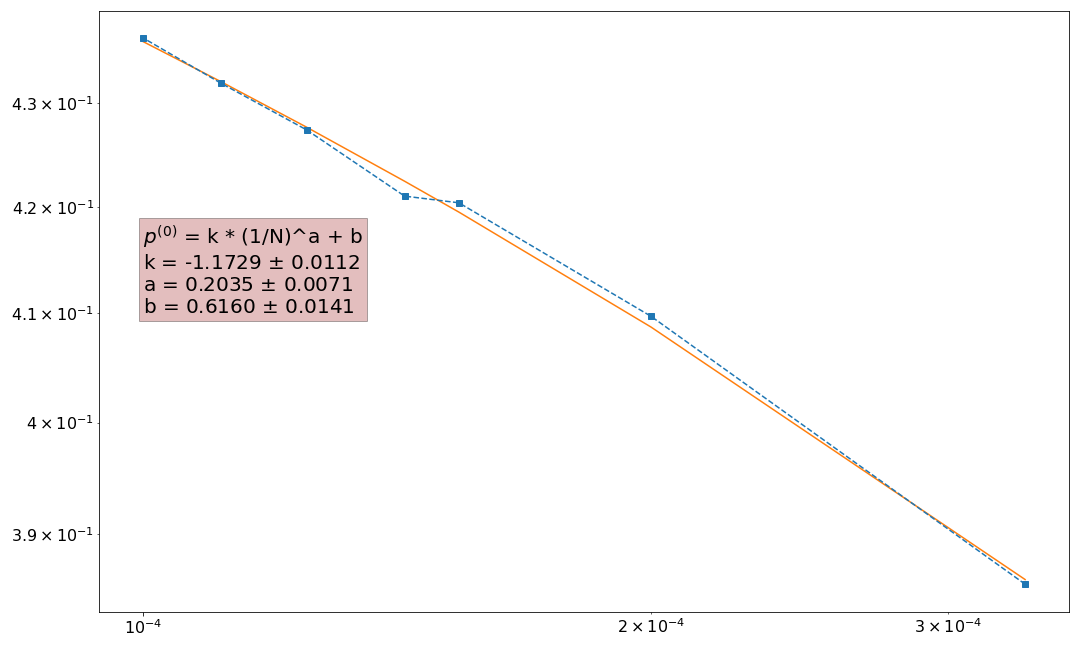
\includegraphics[width=\textwidth]{p0_res.png}
\caption{$p^{(0)}(N)$}
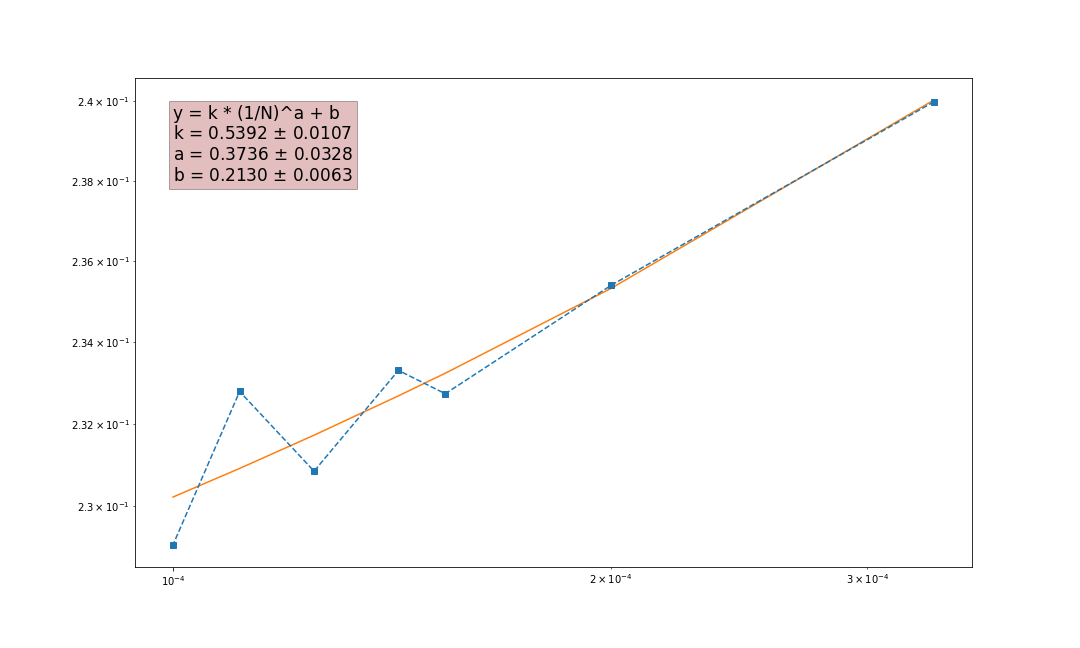
\includegraphics[width=\textwidth]{p1_res.png}
\caption{$p^{(1)}(N)$}
\end{subfigure}
\hfill
\begin{subfigure}{0.495\textwidth}
\centering
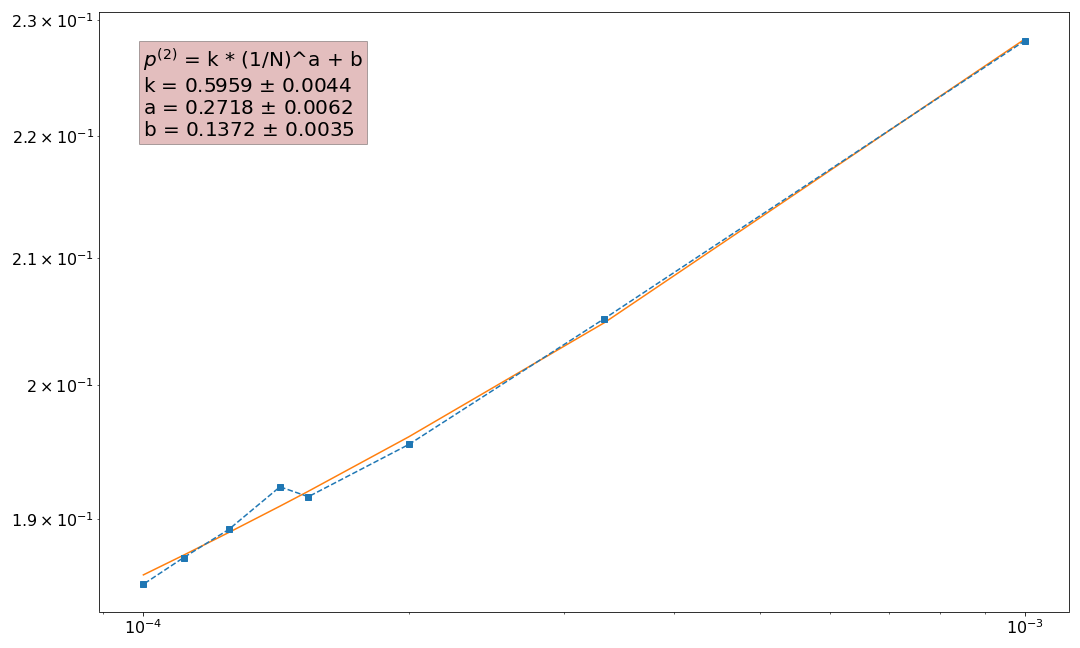
\includegraphics[width=\textwidth]{p2_res.png}
\caption{$p^{(2)}(N)$}
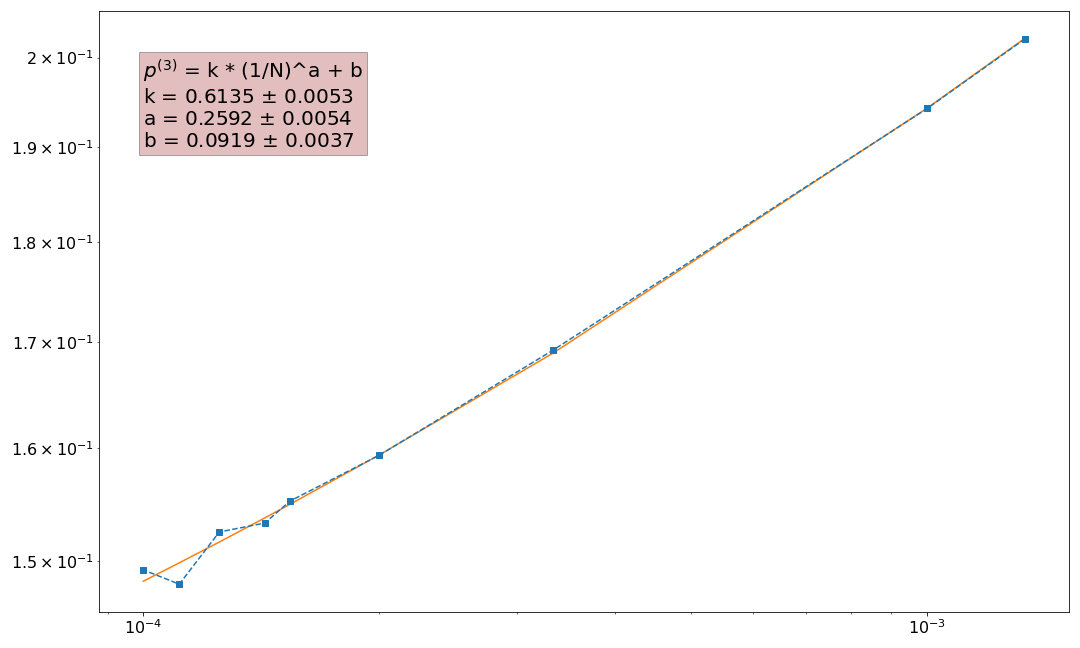
\includegraphics[width=\textwidth]{p3_res.png}
\caption{$p^{(3)}(N)$}
\end{subfigure}
\caption{Вероятности блуждания иметь атмосферу 0-3 от обратной длины конформации в степенном масштабе.}
\label{fig:p_03_loglog}
\end{figure}

Небольшие отклонения графиков апроксимирующей функции от прямолинейного вида обусловлены наличием ненулевого свободного линейного члена,
не входящего в классическую лог-лог регрессию $y = b * x^a$.
Больше всего сомнений вызывает график $p^{(1)}$ в виду сильных колебаний долей блужданий с атмосферой 1 при больших длинах.
Остальные графики $p^{(0)}$, $p^{(2)}$ и $p^{(3)}$ всё же подтверждают степенной (и что наиболее важно, с сильно отличными от нуля степенными коэффициентами) характер сходимости вблизи области бесконечно большой длины.

Интересно, что в данном случае свободные коэффициенты $b_i$ функций от $N$ (таблица \ref{tab:p_i_log_log}) и $\Nun$ (таблица \ref{tab:p_i_u_log_log}) численно очень похожи, в пределах погрешностей. Линейные и степенные коэффициенты, в свою очередь, имеют большие различия, далеко за пределами соотв. погрешностей.

\newpage

\subsection{Общее сравнение поведений атмосфер блужданий и долей узлов простого случайного блуждания}

Для простого случайного блуждания можно отметить сильное по смыслу родство понятий "атмосферы k" блуждания и "доли узлов с i соседями". 
В данном случае очевидно, что если у конца блуждания некоторое число $v$ соседей, то количество незанятых вокруг него узлов всегда равно $4-v$. 
Связь этих свойств гораздо сильнее, чем в случайном блуждании без самопересечений, где для попытки их сопоставления требовалось доп. условие, что блуждание не замкнуто и всегда имеет возможность добавить к себе доп. узел.

Рассмотрим таблицы \ref{tab:n_i_log_log} и \ref{tab:p_i_log_log}, \ref{tab:n_i_u_log_log} и \ref{tab:p_i_u_log_log} на предмет сходства коээфициентов между функциями $\la n_v \ra$ и $\la p^{(4-v)} \ra$.
Сравнение показывает, что между таблицами отсутсвует явная корреляция, за исключением идентичности знаков линейного коээфициента фитирующих функций как от $N$, так и от $N_{unique}$. 

Можно предположить, что связь между ними существует - об этом говорит как подтверждённый степенной характер сходимости, так и схожесть знаков линейных коээфициентов - однако, она крайне слаба ввиду разной статистической мощности наблюдаемых величин - очевидно, что $\la n_v \ra$ охватывает геометрическое поведение всего блуждания, а $\la p^{(v)} \ra$ описывает поведение лишь на его концах, характер которых с увеличением длины блуждания становится некоррелируемым с поведением внутренних узлов.

\newpage

\subsection{Планируемая деятельность}

\begin{itemize}
\item 3-я итерация программного кода для симуляции модели Rand-Walk - добавление в модель аналога квадратной решётки с целью упрощения расчётов уникальных узлов и их соседей.
\end{itemize}
